\section{Measuring Congestion}\label{s:measurement}

\an{shrink this section!}

\name measures network congestion signals (RTT and packet arrival rates) over the duration (or \emph{epochs}) between infrequently sampled packets (that we call \emph{epoch boundary packets}). In this section, we describe our strategy for independently sampling the same set of epoch boundary packets at the paired \name boxes, and for measuring congestion signals using them. We end with an evaluation showing the accuracy of our approach.

\subsection{Determining Epoch Boundaries}
\label{s:measure:marking}

Suppose the desired epoch size, i.e. the number of packets between two epoch boundary packets, is $N$. A naive strategy for determining common epoch boundaries at the \inbox and the \outbox, without making any changes to the packet headers, would be to simply sample a packet after every $N$ packets. However, any packet loss in the network would then desynchronize the sampling at the two boxes.\cut{\footnote{This can be avoided if the \outbox detects and accounts for packet losses, but that would require maintaining expensive per-flow state, which would break our design's simplicity and scalability.}} Another alternative is for the \inbox to explicitly send out-of-band messages to the \outbox indicating which packets are to be sampled. However, there is no guarantee that these messages would arrive at and be processed by the \outbox before the indicated packets arrive themselves. 

Our technique side-steps these issues by using the contents of a packet to sample epoch boundaries. More specifically, a packet is sampled as a boundary for an epoch of size $N$, if the hash over a subset of its fields is a multiple of $N$. Therefore, given sufficient entropy in the hashed values, an epoch boundary will, in expectation, be sampled once every $N$ packets.

\paragrapha{Choosing header subset}
The combination of selected packet fields over which the hash is computed can vary across different deployments, but it must satisfy the following requirements: 

\paragraphn{(i)} It must be the same at both the \inbox and the \outbox.

\paragraphn{(ii)} Its values must remain unchanged as a packet traverses the network from the \inbox to the \outbox (so, for example, the TTL field must be excluded).\footnote{Certain fields, that are otherwise unchanged within the network, can be changed by NATs deployed in a customer's domain. Ensuring that the \name boxes sit outside the NAT would allow them to make use of those fields.}

\paragraphn{(iii)} It differentiates individual \emph{packets} (and not just flows), to allow sufficient entropy in the computed hash values.

\paragraphn{(iv)} It also differentiates a retransmitted packet from the original one, to prevent spurious samples from disrupting the measurements (this precludes, for example, the use of TCP sequence number).

We expect that the precise set of fields used will depend on specific deployment considerations; \ie the tunnelling protocol in use.
For example, in our prototype implementation (\S\ref{s:impl}) we use a ``null'' tunnel with a header subset of the IPv4 IP ID field and destination IP. 
We make this choice for simplicity; it does not require tunnelling mechanisms (and is thus easily deployable); we note that previous proposals~\cite{ip-traceback} have used IP ID for unique packet identification. \radhika{The two major drawbacks of this approach is that it cannot be extended to IPv6 and it is not resilient to scenarios where the \inbox and \outbox see different destination IPs for the same packet (e.g. due to sitting behing a NAT or load balancer).}
A full deployment \radhika{better term?} of \name (which would have to support additional requirements, \eg component IPv6 traffic) could use dedicated fields in the tunnel header such as a VLAN tag \radhika{can we cite something for schemes that have used this before?}.

\subsection{Computing Measurements}
\label{s:measure:compute}
\newcommand{\pone}{$p_{i-1}$}
\newcommand{\hpone}{$h(p_{i-1})$}
\newcommand{\sone}{$s_{i-1}$}
\newcommand{\rone}{$r_{i-1}$}
\newcommand{\ptwo}{$p_{i}$}
\newcommand{\hptwo}{$h(p_{i})$}
\newcommand{\stwo}{$s_{i}$}
\newcommand{\rtwo}{$r_{i}$}
\newcommand{\atwo}{$a_{i}$}
\newcommand{\sentone}{$sent_{i-1}$}
\newcommand{\recvdone}{$rcvd_{i-1}$}
\newcommand{\senttwo}{$sent_{i}$}
\newcommand{\recvdtwo}{$rcvd_{i}$}


\begin{figure}
    \centering
    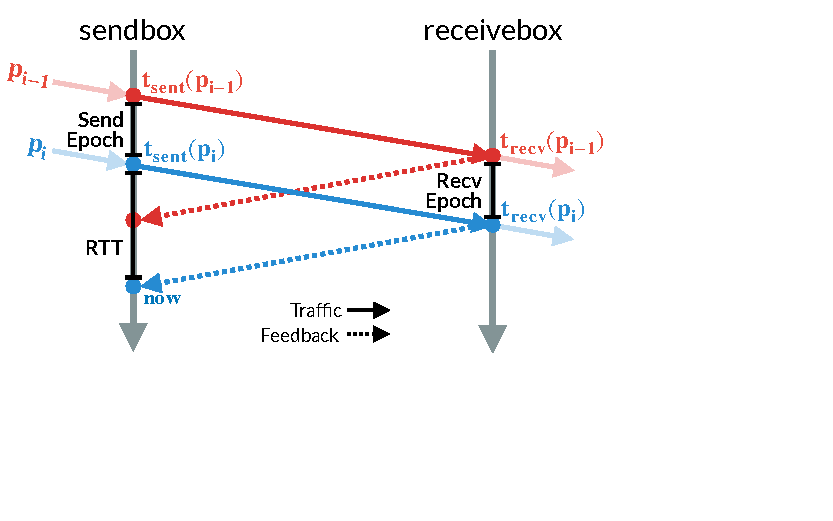
\includegraphics[width=\columnwidth]{img/rate-calculation}
    \caption{Example of epoch-based measurement calculation. Time moves from top to bottom.
    %Packets from flows in a bundle
    %pass through the \inbox and \outbox middleboxes on the way to their destination. 
    The \inbox records the packets that are identified as epoch boundaries. 
    The \outbox, up on identifying such packets, sends a feedback message back to
    the \inbox, which allows it to calculate the RTT and epochs.
    %When the \inbox observes a packet header matching the boundary condition, it records it. 
    %When the \outbox observes this packet, it sends an out-of-band feedback message back to
    %the \inbox, which allows it to calculate the RTT and epochs.
    }\label{fig:ratecalc}
\end{figure}

Given our technique to identify epoch boundaries, it is straight-forward to measure congestion signals, as illustrated in Figure~\ref{fig:ratecalc}.
For each bundle, the \inbox tracks the total number of bytes sent within this bundle, and, upon identifying an epoch boundary packet, $p_i$, it records: (i) its hash, $h(p_i)$, (ii) the time when it is sent out, $t_{\text{sent}}(p_i)$, and (iii) the total number of bytes sent thus far including this packet, $b_{sent}(p_i)$. 

The \outbox similarly tracks the total number of bytes received for each bundle. Upon the arrival and identification of the epoch boundary packet $p_i$, it immediately sends a feedback message to the \inbox containing: (i) its hash, $h(p_i)$, (ii) the time when it was received, $t_{recv}(p_i)$, and (iii) the total number of bytes received thus far including this packet, $b_{recv}(p_i)$. 

Upon receiving the feedback $p_i$, the \inbox records the received information, and using its previously recorded state, it can compute the RTT and the rates at which packets are sent and received, as below:

% \begin{subequations}
%     \begin{align}
%         RTT &= &now - s_2 \\
%         \cut{
%         send\_epoch\_duration &= &s_2 - s_1\\
%         recv\_epoch\_duration &= &r_2 - r_1\\
%         bytes\_sent\_in\_epoch &= &bytes\_sent\ at\ s_2 &\ - \\
%                                     &&bytes\_sent\ at\ s_1&\notag\\
%         bytes\_rcvd\_in\_epoch &= &bytes\_rcvd\ at\ r_2 &\ - \\
%                                 &&bytes\_rcvd\ at\ r_1\notag\\
%         send\_rate &= &\frac{bytes\_sent\_in\_epoch}{send\_epoch\_duration}\\
%         recv\_rate &= &\frac{bytes\_rcvd\_in\_epoch}{recv\_epoch\_duration}
%         }
%         send\_rate &= &\frac{bytes\_sent\ at\ s_2 - bytes\_sent\ at\ s_1}{s_2-s_1}\\
%         recv\_rate &= &\frac{bytes\_rcvd\ at\ r_2 - bytes\_rcvd\ at\ r_1}{r_2-r_1}
%     \end{align}
% \end{subequations}
\vspace{-10pt}
\begin{subequations}
    \begin{align}
        RTT &= &now -  t_{sent}(p_i)\\
        send\_rate &= &\frac{b_{sent}(p_i) - b_{sent}(p_{i-1})}{t_{sent}(p_i)-t_{sent}(p_{i-1})}\\
        recv\_rate &= &\frac{b_{recv}(p_i) - b_{recv}(p_{i-1})}{t_{recv}(p_i)-t_{recv}(p_{i-1})}
    \end{align}
\end{subequations}

Finally, the \inbox clears the recorded state of all epoch boundaries preceding $p_i$.

Note that our measurement technique is robust to a boundary packet being lost between the \inbox and the \outbox. In this case, the \inbox would not get a feedback for the lost boundary packet, and it would simply compute rates for the next boundary packet over a longer epoch. 

% \paragrapha{Crashes \an{need better heading}} Existing work~\cite{ftmb} has studied how to design stateful middleboxes to be fault-tolerant with acceptable performance overheads. 
% However, state-persistence is largely unnecessary for \name.
% \name only stores network conditions, which it can re-learn within a few RTTs, and bundle membership flow tables, which it can re-discover as we describe in~\S\ref{s:impl:discovery}. 
% \radhika{maybe move elsewhere}

\subsection{Choosing The Epoch Size}
\label{s:measure:epoch}
%\begin{figure}
    \centering
\begin{knitrout}
\definecolor{shadecolor}{rgb}{0.969, 0.969, 0.969}\color{fgcolor}
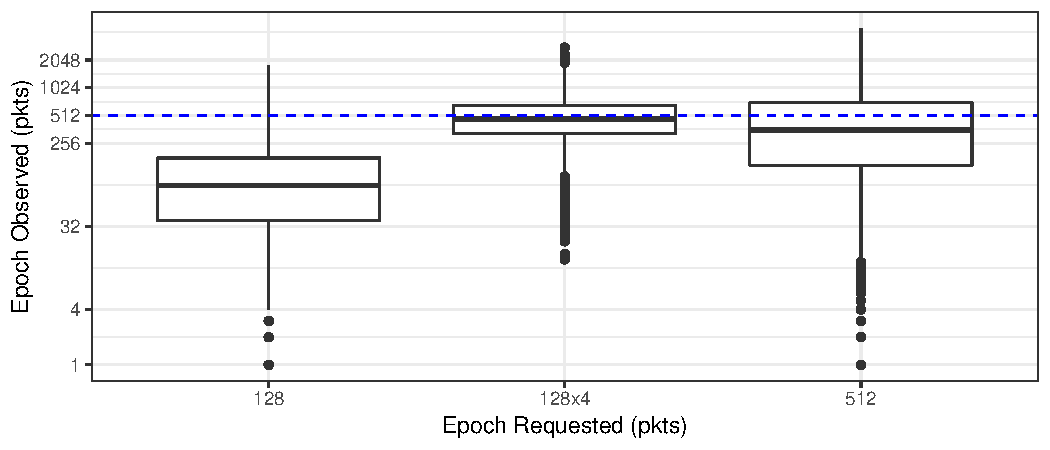
\includegraphics[width=\maxwidth]{figure/micro:epoch-1} 

\end{knitrout}
    \caption{Distribution of observed epoch sizes based on the desired epoch size. Suppose we
    need an epoch size of 512. By setting the epoch size to $\frac{1}{4}$ of that and using
    a sliding window over the last 4 epochs, we can achieve the same average epoch size with
    significantly lower variance than if we were to set the epoch size to 512 directly.
    \fc{todo: real eval data}}
    \label{fig:micro:epoch}
\end{figure}


% How do we choose the number of packets that should e in each epoch?
In \S\ref{s:measure:marking}, we assumed a fixed epoch size of $N$ packets. However, in practice, epochs must be such that measurements are collected at least once per RTT~\cite{ccp}. Therefore, for each bundle, we track that minimum observed RTT ($minRTT$) at the \inbox and set the epoch size $N = (0.25 \times minRTT \times send\_rate)$, where the $send\_rate$ is compute as described above. The final rates passed to the congestion control algorithms at the \inbox are then computed over a sliding window of epochs that corresponds to one RTT. Averaging over a window of multiple epochs also increases resilience to possible re-ordering of packets between the \inbox and the \outbox, which can result in them seeing different number of packets between two epochs.
%This makes epoch size a function of the bandwidth-delay product (BDP).
% Because epoch sizes are sampled from a uniform random variable, setting larger epoch sizes will increase the variance in the observed epoch sizes.
% If the epoch size is small relative to the rate, the raw measurements will be noisy, but we can correct for this by measuring over a sliding window.

% How do we choose the number of packets that should e in each epoch?
% In \S\ref{s:measure:marking}, we assumed a fixed epoch size of $N$ packets.
% However, in practice, the epoch must be a function of the bandwidth-delay product (BDP).
% Because epoch sizes are sampled from a uniform random variable, setting larger epoch sizes will increase the variance in the observed epoch sizes.
% If the epoch size is small relative to the rate, the raw measurements will be noisy, but we can correct for this by measuring over a sliding window.

% Therefore, we estimate the BDP (current sending rate multiplied by current estimate of the RTT) and set the desired epoch size to one-fourth of this value. We then calculate rates over a sliding window of four epochs; this is approximately one RTT.


When the \inbox updates the epoch size $N$ for a bundle, it needs to send an out-of-band message to the \outbox communicating the new value. To keep our measurement technique resilient to potential delay and loss of this message, the epoch size $N$ is always rounded down to the nearest power of two. Doing this ensures that the epoch boundary packets sampled by the \outbox are either a strict superset or a strict subset of those sampled by the \inbox. The \inbox simply ignores the additional feedback messages in former case, and the recorded epoch boundaries for which no feedback has arrived in the latter.  

%As the sending rate and RTT change, the \inbox will update the desired epoch size accordingly, and communicate this desired epoch size to the \outbox.
% This communication might be lost. 
% Therefore, when setting the desired epoch size we round down to the nearest power of two so that the \outbox's view of the epoch boundary packets is a sub- or super- set of the \inbox's:
% for example, 
% if the \inbox's desired epoch size is $64$ packets
% but the \outbox does not receive this update and still believes the desired epoch size is $128$ packets, 
% the \outbox's feedback will still match (in expectation) half the \inbox's epoch boundary packets.


% \subsection{Dealing with packet re-ordering and losses}

% \Para{Packet Loss} Our technique is robust to loss of boundary packets between the \inbox and the \outbox.
% Suppose the \inbox sees boundary packets $p_1, p_2, p_3$, but $p_2$ is lost after passing through
% the \inbox so the \inbox only receives feedback for $p_1$ and $p_3$. Upon receiving $p_1$, 
% the \inbox will truncate its data structure up until $p_1$. Upon receiving $p_3$, the \inbox 
% looks up the oldest remaining boundary packet, $p_1$, and considers that the beginning of the epoch.
% As a result, the epoch is longer than expected, but no measurements are lost or corrupted. 
% The same argument applies to the loss of feedback messages. 
% Importantly, \inbox calculates both the send and receive epoch based on information
% from the \outbox rather than attempting to reach consensus on individual epoch boundaries with the \outbox.

% \Para{Packet loss} This method is robust to the loss of boundary packets between the \inbox and \outbox.
% Suppose the \inbox sees boundary packets $p_1, p_2, p_3$, but $p_2$ is lost after passing through
% the \inbox so the \inbox only receives feedback for $p_1$ and $p_3$. Upon receiving $p_1$, 
% the \inbox will truncate its data structure up until $p_1$. Upon receiving $p_3$, the \inbox 
% looks up the oldest remaining boundary packet, $p_1$, and considers that the beginning of the epoch.
% As a result, the epoch is longer than expected, but no measurements are lost or corrupted. 
% The same argument applies to the loss of feedback messages. 
% Importantly, \inbox calculates both the send and receive epoch based on information
% from the \outbox rather than attempting to reach consensus on individual epoch boundaries with the \outbox. 

%\Para{Re-Ordering}
%\label{s:measure:limitation:reorder}

% Earlier we ignored re-ordering of packets between the \inbox and \outbox. However, if packets
% are re-ordered, the \inbox and \outbox will observe a different view of the same epoch.
% For example, consider packets numbered 1 to 20, where 10 is a boundary packet. The \inbox observes
% 10 packets in each epoch: [1,10] in epoch 1 and [11,20] in epoch 2. 
% However, suppose packet 7 is delayed and arrives after packet 10. The \outbox will observe 9
% packets in epoch 1 and 11 packets in epoch 2. 
% Spurious re-ordering can be compensated by using an EWMA across epochs rather than the raw values
% calculated at each epoch. If there is persitent re-ordering, it may be necessary to add a constant 
% value to either the send or receive rate to compensate.
%\radhika{the explanation seems a bit hand-wavy. if we end up doing ecmp expt and the results look good, add fwd pointer to those results}



% \subsubsection{Suitable Algorithms}
% \label{s:measure:limitation:algs}
% The set of measurements we obtain are sufficient for most rate-based algorithms, but may not be 
% suitable for traditional window-based algorithms which require low-level metrics such as 
% the number of inflight packets or number of packets lost. Although it should be possible
% to compute these from the measurements we already collect in an ideal scenario, they would easily
% break in the presence of network anomilies such as re-ordering. Thus, we leave the development
% of robust signals for window-based algorithms to fuure work. 
% Thus, \name currently operates best with rate-based algorithms such as BBR, Nimbus, or Copa~\cite{bbr,nimbus,copa}.
% \radhika{feels like this should be moved to Sec 3, but am  not entirely sure.}
% \radhika{discuss}

\subsection{Microbenchmarks}
\label{s:measure:microbench}
    \begin{figure}
    \centering
\begin{knitrout}
\definecolor{shadecolor}{rgb}{0.969, 0.969, 0.969}\color{fgcolor}\begin{kframe}


{\ttfamily\noindent\color{warningcolor}{\#\# Warning in file(file, "{}rt"{}): cannot open file 'minrtt-50-delay-dist.out': No such file or directory}}

{\ttfamily\noindent\bfseries\color{errorcolor}{\#\# Error in file(file, "{}rt"{}): cannot open the connection}}

{\ttfamily\noindent\bfseries\color{errorcolor}{\#\# Error in `colnames<-`(`*tmp*`, value = c("{}t"{}, "{}mm\_delay"{}, "{}inbox\_delay"{}, : attempt to set 'colnames' on an object with less than two dimensions}}

{\ttfamily\noindent\bfseries\color{errorcolor}{\#\# Error in data\$t: object of type 'closure' is not subsettable}}

{\ttfamily\noindent\bfseries\color{errorcolor}{\#\# Error in eval(expr, envir, enclos): object 'p1' not found}}\end{kframe}
\end{knitrout}

\begin{knitrout}
\definecolor{shadecolor}{rgb}{0.969, 0.969, 0.969}\color{fgcolor}\begin{kframe}


{\ttfamily\noindent\color{warningcolor}{\#\# Warning in file(file, "{}rt"{}): cannot open file 'minrtt-delay-dist.out': No such file or directory}}

{\ttfamily\noindent\bfseries\color{errorcolor}{\#\# Error in file(file, "{}rt"{}): cannot open the connection}}

{\ttfamily\noindent\bfseries\color{errorcolor}{\#\# Error in `colnames<-`(`*tmp*`, value = c("{}t"{}, "{}mm\_delay"{}, "{}inbox\_delay"{}, : attempt to set 'colnames' on an object with less than two dimensions}}

{\ttfamily\noindent\bfseries\color{errorcolor}{\#\# Error in data\$diff\_delay: object of type 'closure' is not subsettable}}

{\ttfamily\noindent\bfseries\color{errorcolor}{\#\# Error in data\$diff\_delay: object of type 'closure' is not subsettable}}

{\ttfamily\noindent\bfseries\color{errorcolor}{\#\# Error in data\$diff\_delay: object of type 'closure' is not subsettable}}

{\ttfamily\noindent\bfseries\color{errorcolor}{\#\# Error in data.frame(x = dens\_delay\$x, y = dens\_delay\$y): object 'dens\_delay' not found}}

{\ttfamily\noindent\bfseries\color{errorcolor}{\#\# Error in data\$diff\_delay: object of type 'closure' is not subsettable}}

{\ttfamily\noindent\bfseries\color{errorcolor}{\#\# Error in is.unsorted(vec): object 'quants\_delay' not found}}

{\ttfamily\noindent\bfseries\color{errorcolor}{\#\# Error in which(df\_delay\$quant == 1): object 'df\_delay' not found}}

{\ttfamily\noindent\bfseries\color{errorcolor}{\#\# Error in eval(expr, envir, enclos): object 'df\_delay' not found}}

{\ttfamily\noindent\bfseries\color{errorcolor}{\#\# Error in eval(expr, envir, enclos): object 'df\_delay' not found}}

{\ttfamily\noindent\bfseries\color{errorcolor}{\#\# Error in eval(expr, envir, enclos): object 'quants\_delay' not found}}

{\ttfamily\noindent\bfseries\color{errorcolor}{\#\# Error in rbind(df\_delay, c(quants\_delay[["{}10\%"{}]] - 1e-04, med, 0)): object 'df\_delay' not found}}

{\ttfamily\noindent\bfseries\color{errorcolor}{\#\# Error in rbind(df\_delay, c(quants\_delay[["{}10\%"{}]] + 1e-04, med, 1)): object 'df\_delay' not found}}

{\ttfamily\noindent\bfseries\color{errorcolor}{\#\# Error in which(df\_delay\$quant == 2): object 'df\_delay' not found}}

{\ttfamily\noindent\bfseries\color{errorcolor}{\#\# Error in eval(expr, envir, enclos): object 'df\_delay' not found}}

{\ttfamily\noindent\bfseries\color{errorcolor}{\#\# Error in eval(expr, envir, enclos): object 'df\_delay' not found}}

{\ttfamily\noindent\bfseries\color{errorcolor}{\#\# Error in eval(expr, envir, enclos): object 'quants\_delay' not found}}

{\ttfamily\noindent\bfseries\color{errorcolor}{\#\# Error in rbind(df\_delay, c(quants\_delay[["{}90\%"{}]] - 1e-04, med, 1)): object 'df\_delay' not found}}

{\ttfamily\noindent\bfseries\color{errorcolor}{\#\# Error in rbind(df\_delay, c(quants\_delay[["{}90\%"{}]] + 1e-04, med, 2)): object 'df\_delay' not found}}

{\ttfamily\noindent\bfseries\color{errorcolor}{\#\# Error in data\$diff\_delay: object of type 'closure' is not subsettable}}

{\ttfamily\noindent\bfseries\color{errorcolor}{\#\# Error in ggplot(df\_delay, aes(x, y)): object 'df\_delay' not found}}

{\ttfamily\noindent\bfseries\color{errorcolor}{\#\# Error in eval(expr, envir, enclos): object 'p\_delay' not found}}\end{kframe}
\end{knitrout}

    \caption{\name's estimate of the delay }
    \label{fig:micro:time-delay}
\end{figure}
 % actually contains the distributions
    \begin{figure}
    \centering
\begin{knitrout}
\definecolor{shadecolor}{rgb}{0.969, 0.969, 0.969}\color{fgcolor}
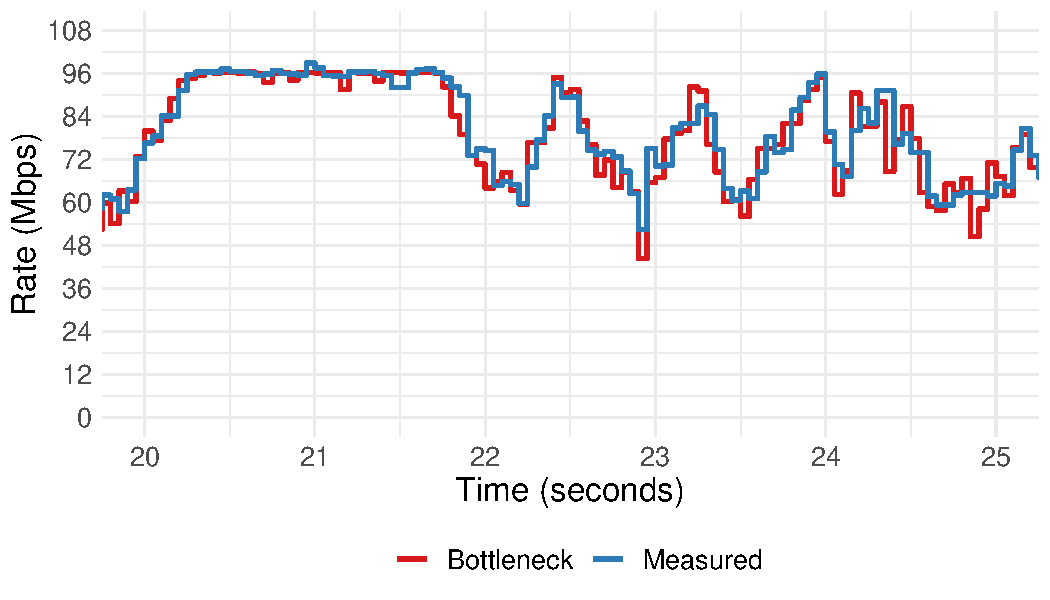
\includegraphics[width=\maxwidth]{figure/micro:time-thru-1} 

\end{knitrout}

    \caption{\name's estimate of the receive rate.}
    \label{fig:micro:time-thru}
\end{figure}
 % actually contains the time series
    We now evaluate the accuracy of our measurement technique and its robustness to various network conditions. 

    We pick 90 traces of \name's measurements from experiments in our evaluation across a range of RTTs (20ms, 50ms, 100ms) and bottleneck rates (24Mbps, 48Mbps, 96Mbps) and compute the difference between our measured value of the RTT and receive rate at each time step compared to the values at the bottleneck router. We plot the distribution of these differences for all of the traces in Figure~\ref{fig:micro:time-delay}. 80\% of our RTT estimates are within 1.2ms of the actual value and 80\% of our receive rate estimates are within 4Mbps of the actual value. 
    
    To visualize how these measurements impact the behavior of the signals over time we pick an experiment for which the median difference matches that of the entire distribution and plot a five second segment of our estimates compared to the actual values in Figure~\ref{fig:micro:time-thru}.
